\documentclass[12pt]{article}
\usepackage[left=3.3cm,right=3.3cm,bottom=3.0cm,top=3.0cm]{geometry}
\usepackage{float}
\usepackage{graphicx}
\usepackage{tikz}
\usepackage{subcaption}
\usepackage{algorithm}
\usepackage{algorithmic}
\usepackage{comment}
\usepackage{mathptmx}
\usepackage{microtype}
\usepackage{array}
%\usepackage{amsthm}

\usetikzlibrary{arrows}

%\floatstyle{boxed}
%\restylefloat{figure}

%\theoremstyle{definition}
%\newtheorem{definition}{Definition}

\newcommand{\LengthVar}{L}
\newcommand\Base[1]{{\tt #1}}
\newcommand{\ReadArrowType}{latex}
\newcommand{\Figure}[1]{Figure \ref{#1}}
\newcommand{\Subfigure}[1]{Figure \ref{#1}}
\newcommand{\Section}[1]{Section \ref{#1}}
\newcommand{\Subsection}[1]{Section \ref{#1}}
\newcommand{\Algorithm}[1]{Algorithm \ref{#1}}

\newcommand{\KeyTerm}[1]{{\it #1}}
\newcommand{\ProgramName}[1]{{\tt #1}}
\newcommand{\BidirectedEdgeForward}[2]{
		\tikz[>=triangle 45,baseline]
		\draw[>->,thin] (0,0.1) node[anchor=east] {#1} --
					    (0.8,0.1) node[anchor=west] {#2};}

\title{A Bidirected String Graph Model for Genome Assembly}
\author{Eric Biggers}


\begin{document}
\maketitle

\begin{abstract}

Sequencing an organism's genome is an important step to further genetic research
on that organism.  However, currently available sequencing technologies can only
sequence short fragments of DNA.  As a result, the whole-genome shotgun
sequencing approach to genome sequencing relies on breaking up a sample of
genomic DNA into fragments, sequencing these fragments, then using a program
called a {\em genome assembler} to put together these short sequences to
reconstruct the original, much longer sequence.  This paper provides an
introduction and formalization of the genome assembly problem, then introduces a
model and algorithm for genome assembly that is based on a special type of graph
called a \KeyTerm{bidirected string graph}.  \end{abstract}

\tableofcontents

\section{Introduction to genome sequencing and assembly}

\subsection{Definition of a genome}

Every living organism contains a collection of hereditary material called a
\KeyTerm{genome}.  Typically, each cell of a multicellular organism contains a
complete copy of that organism's genome.  A genome consists of one or more DNA
(\KeyTerm{deoxyribonucleic acid}) molecules in the form of
\KeyTerm{chromosomes}.  DNA is a double-stranded molecule, each strand of which
is a polymer of \KeyTerm{nucleotides}.  A nucleotide, together with the
corresponding nucleotide on the opposite strand, is called a \KeyTerm{base pair}
(abbreviation: \KeyTerm{bp}).  In DNA, there are four possible nucleotides:
adenine, cytosine, guanine, and thymine, which are abbreviated as \Base{A},
\Base{C}, \Base{G}, and \Base{T}, respectively.  \Base{A} always pairs with T on
the opposite strand, and \Base{C} always pairs with \Base{G} on the opposite strand.
In addition, each strand has a direction, and the two strands of a DNA molecule
are directed opposite one another.  Furthermore, a DNA molecule may be circular,
as is usually the case for bacterial chromosomes.

Based on these biological facts, a genome is formally defined, for the purposes
of this paper, as a set of possibly circular, dual-stranded strings of the
symbols \Base{A}, \Base{C}, \Base{G}, and \Base{T}, where dual-stranded has the
meaning indicated above (the two strands run in opposite directions, and the
pairings \Base{A}---\Base{T} and \Base{C}---\Base{G} always hold).

This definition does not account for the fact that the genomes of diploid and
polyploid organisms, including most plants and animals, contain multiple
slightly-differing copies of each chromosome.  In this case, the above
definition will consider each copy of each chromosome to be a completely
different string in the genome, unless the copies are completely identical.

Genomes vary widely in size, from several thousand base pairs to many billion
base pairs, depending on the organism (see Table \ref{tab:GenomeSizes}).

\begin{table}[H]
	\begin{center}
		\begin{tabular}{|c|>{\centering\arraybackslash}p{5.2cm}|}
			%\hline
			%$\phi$X174 bacteriophage &  $\sim$5,000 bp \\
			%\hline
			%Human mitochondrion &  $\sim$16,000 bp \\
			\hline
			{\bf Organism} & {\bf Approximate genome size} \\
			\hline
			{\it Variola} virus (smallpox) &  186,000 bp\\
			\hline
			{\it E. coli} (a bacterium) & 4,600,000 bp \\
			\hline
			{\it Ananas comosus} (domesticated pineapple) & 500,000,000 bp \\
			\hline
			{\it Zea mays} (domesticated corn) & 2,000,000,000 bp \\
			\hline
			{\it Homo sapiens} (human)       &  3,200,000,000 bp \\
			\hline
		\end{tabular}
	\end{center}
	\caption{Approximate genome sizes of selected organisms}
	\label{tab:GenomeSizes}
\end{table}

\subsection{Complement and reverse-complement sequences}

The \KeyTerm{complement} of a single-stranded DNA sequence $S$ is the
single-stranded DNA sequence obtained by making the replacements $\Base{A}
\leftrightarrow \Base{T}$ and $\Base{C} \leftrightarrow \Base{G}$.  The
\KeyTerm{reverse-complement} of a single-stranded DNA sequence $S$ is the
complement of $S$ reversed.  Physically, the reverse-complement of a
single-stranded DNA sequence corresponds to the corresponding sequence on the
other strand of the DNA molecule.  It is the reverse-complement, not the
``regular'' complement, because the two strands of a DNA molecule run in
opposite directions.

The \KeyTerm{canonical form} of a DNA sequence $S$ is the lexicographically
lesser of $S$ and its reverse-complement $S'$.  This concept is useful in
algorithms where a DNA sequence and its reverse-complement are considered
equivalent.

\subsection{Genome sequencing}

\KeyTerm{DNA sequencing} is the process of determining the base pair sequence of
(\KeyTerm{sequencing}) one or more DNA molecules.  \KeyTerm{Genome sequencing}
is the use of DNA sequencing to determine the base pair sequence of an entire
genome.

Sequencing a DNA molecule is very difficult because it is in fact an actual
molecule, which makes each base pair much too small to be directly observed.
Therefore, indirect laboratory techniques must be used.  Advances in these
techniques are progressing rapidly, and they can now be performed by automated
machines.  However, every technique suffers from the limitation that only short
fragments of DNA several dozen to several thousand base pairs long can be
sequenced.

Therefore, to sequence an entire genome, which may be millions of base pairs
long, the DNA from the whole genome must be broken into much smaller fragments,
which are then sequenced.\footnote{This specifically refers to the
\KeyTerm{whole-genome shotgun sequencing} approach to genome assembly rather
than alternatives such as \KeyTerm{BAC-to-BAC} sequencing that are able to
restrict sequences to certain regions of the genome in order to make sequencing
the genome easier (currently, at the disadvantage of increased cost and
non-computational work).} Following this, the original genome must be
computationally reconstructed by a computer program called a \KeyTerm{genome
assembler} in a process called \KeyTerm{genome assembly}.  \KeyTerm{Genome
sequencing} therefore refers to the entire process of sequencing a genome,
including both lab work and computational work, while \KeyTerm{genome assembly}
only refers to the computational work.\footnote{It usually also takes some
technology-specific computational work to actually prepare the sequences for
assembly; for example, a series of digital photographs of clumps of
fluorescently labeled molecules might need to be interpreted as reads using
image-processing algorithms.  However, these programs and/or algorithms
generally have already been developed by the manufacturer of the sequencing
machine and work fairly well, and ``genome assembly'' does not cover these
algorithms, although assemblers still may be tuned for specific sequencing
technologies.}

\subsection{Genome assembly}

\label{subsec:reads}

The goal of genome assembly is to reconstruct a genome, as defined earlier,
given a set of substrings that may originate from any strand of any DNA molecule
in the genome.  Each substring is called a \KeyTerm{read} and is the sequence of
some DNA that was sequenced by the sequencing machine.  In general, reads may
contain errors, including \KeyTerm{substitutions}, where a base pair in the read
was incorrectly read as some other base pair, as well as \KeyTerm{insertions},
where a sequence of one or more random base pairs have been inserted into some
position in the read, and \KeyTerm{deletions}, where a sequence of one or more
base pairs from the original genome is missing from the interior of the read.
Reads are expected to be uniformly distributed on the genome with a certain
coverage $X$ depending on how much data was collected, meaning that each base
pair in the original genome is expected to be included in $X$ different reads on
average, allowing for the reads to be from either strand.  However, some
sequencing technologies produce biased data where the coverage across the genome
is much more variable than that expected by uniform, random sampling.

Reads may contain other information, such as \KeyTerm{quality scores} or
\KeyTerm{mate-pair} information, that can provide additional hints to the
assembler.

It is also possible for reads to come from foreign DNA; for example, if a DNA
sample is obtained from grinding up plant or animal tissue, there could be some
bacterial cells, each with its own genome, contaminating the sample.  Ideally,
an assembler should be prepared to completely ignore a read if it seems too
unusual.  However, this problem is not considered in this paper.

For the purposes of this paper, the problem of genome assembly is simplified by
assuming the following characteristics of the reads:

\begin{itemize}
	\item The reads are error-free and uniformly sampled from the genome.
	\item There are no reads from foreign DNA.
	\item The reads are unpaired, meaning that mate-pair information, if
available, is not used.
\end{itemize}

In other words, a read is defined here as an exact substring from either strand
of any part of the genome.

Genomes may contain \KeyTerm{repeats}, which are subsequences that occur
multiple times in the genome--- possibly adjacent to each other (a
\KeyTerm{tandem repeat}), but not necessarily.  Repeats may be longer than the
length of any individual read, which makes the genome more difficult to assemble
accurately.  However, real genomes almost always contain repeats of substantial
length, so assemblers must be able to handle repeats.

\subsection{Genome assembly vs. shortest common superstring}

Genome assembly is superficially similar to the shortest common superstring
problem, which is to find the shortest possible string that contains every
string in a given set as substrings.  Genome assembly also requires finding a
longer string that, roughly, contains every string in  a set of substrings.
However, the actual genome may be more than one string, and the genome may also
be longer than the shortest possible genome from which the reads could have been
sampled, due to repeats.  In addition,  genomes are double-stranded, and there
may be other complications with the reads, such as sequencing error.  Therefore,
genome assembly is not the same as the shortest common superstring problem, and
in fact seems to be harder, despite the fact that the shortest common
superstring problem is already NP-complete\cite{Turner1989}.

In fact, some models of genome assembly have also been proven to be
NP-complete\cite{Medvedev2007}.  However, it is not acceptable to have a genome
assembly algorithm that takes exponential time to complete.  Instead, heuristic
algorithms that tend to produce good results on real inputs while still having
reasonable running times must be designed.

\section{Overview of the fragment string graph algorithm}

This paper explores the genome assembly problem through an algorithm published
in 2005 by Eugene Myers that is based on the idea of the fragment string
assembly graph\cite{Myers2005}.  The algorithm provides a good overview of the
techniques that are used in genome assembly, especially since it draws on ideas
used in previous assemblers, such as the Celera assembler, which was used to
assemble the human genome for the first time\cite{Venter2001}.  In addition, the
algorithm shares some ideas with de Bruijn graph-based assemblers, such as
EULER-SR\cite{Pevzner2001}, although it does not use a de Bruijn graph for its
assembly model.  In fact, the algorithm is called the {\em fragment} string
graph algorithm because the graph is built directly from the sequenced fragments
(or reads), rather than subsequences ($k$-mers) taken from them.

The algorithm also introduces new ideas that were not used in previous
publications or assemblers.

The overall fragment string graph algorithm can be described as follows.  First,
use overlaps between reads to build a graph that models the assembly problem.
The idea is that walks through this graph model a way in which reads may be
assembled together consistently when the overlaps are used as evidence for
joining pairs of reads.  The next step is to simplify and analyze the graph, and
the last step is to find paths through the graph to reconstruct the original
genome.\footnote{The fragment string graph algorithm, as described in
\cite{Myers2005}, does not involve any finishing steps such as scaffolding
(using mate-pair information to improve the assembly), although ideas for doing
this are outlined in \cite{Medvedev2009}.  However, in this paper we assume that
no mate-pair information is available.}

\section{Overlaps}

\subsection{Definition of an overlap}
%\begin{definition}
	Consider two reads, $f$ and $g$, and their reverse-complements $f'$ and
	$g'$.  The reads $f$ and $g$ are said to \KeyTerm{exactly overlap} by some
	length $\LengthVar$ if and only if at least one of the following is true:
	\begin{itemize}
		\item The last $\LengthVar$ bp of $f$ exactly match the first
		$\LengthVar$ bp of $g$.
		\item The last $\LengthVar$ bp of $f$ exactly match the first
		$\LengthVar$ bp of $g'$.
		\item The last $\LengthVar$ bp of $f'$ exactly match the first
		$\LengthVar$ bp of $g$.
		\item The last $\LengthVar$ bp of $f'$ exactly match the first
		$\LengthVar$ bp of $g'$.
	\end{itemize}
%\end{definition}

Having four different conditions is required because reads may overlap in a
reverse-complement manner.  An overlap is reverse-complement if and only if one
read in the overlap is used in the original direction and the other read is used
in the reverse-complement direction.  Note that an overlap from condition (4) is
{\em not} a reverse-complement overlap, as it can equivalently be stated as the
last $\LengthVar$ bp of $g$ exactly match the last $\LengthVar$ bp of $f$.
\Figure{fig:overlap_types} shows the three fundamental types of overlaps that
may arise from this definition.

A read may overlap with itself; for example, a read may contain a suffix that
matches its prefix of the same length.  Such an overlap is called a
\KeyTerm{self-overlap}.

Overlaps may also be \KeyTerm{inexact}.  An inexact overlap is an overlap where
overlapped regions of the two reads do not match exactly (in either a forward or
reverse-complement manner), but instead differ by a number of base-pair
substitutions, insertions, and/or deletions up to a predetermined upper bound,
such as 5\%.  However, inexact overlaps will not be considered further in this
paper.

An overlap $o$ is fully described by the 7-tuple $(f,\ f_{begin},\ f_{end},\ g,
\ g_{begin},\ g_{end},\ rc)$, where $f$ and $g$ are the two reads involved in the
overlap, $f_{begin}$ and $f_{end}$ are the starting and ending indices of the
overlapped region on the $f$ read, $g_{begin}$ and $g_{end}$ are the starting
and ending indices of the overlapped region on the $g$ read, and $rc$ is a
boolean that indicates whether the overlap is reverse-complement or not.  An
overlap therefore has two overlapped regions--- one on each read.  For exact
overlaps, the two overlapped regions are the same length; in other words,
$g_{end} - g_{begin} = f_{end} - f_{begin}$.

An \KeyTerm{extreme point} occurs when an overlapped region extends to the
beginning or the end of the corresponding read.  An overlap always contains at
least two extreme points.

A \KeyTerm{containing overlap} is an overlap in which the overlapped region of
one read, the \KeyTerm{contained read}, is the entire read.  A special case of a
containing overlap is an overlap where the overlapped regions include the
entirety of both reads.  For an exact overlap, this can only happen if the two
reads are either identical or exact reverse-complements of each other.

\begin{figure}
	\centering
	\begin{subfigure}[b]{0.3\textwidth}
		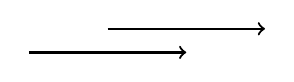
\begin{tikzpicture}=\ReadArrowType]
			\draw[->,style=thick] (0,0) -- (2,0);
			\draw[->,style=thick] (1.0,0.3) -- (3.0,0.3);
		\end{tikzpicture}
		%\vspace{3mm}
		%or (symmetrically)
		%\vspace{3mm}

		%\begin{tikzpicture}=\ReadArrowType]
			%\draw[->,style=thick] (2,0) -- (0,0);
			%\draw[->,style=thick] (3.0,0.3) -- (1.0,0.3);
		%\end{tikzpicture}
		\caption{``Normal'' overlap}
	\end{subfigure}
	\begin{subfigure}[b]{0.3\textwidth}
		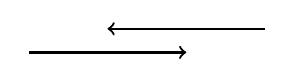
\begin{tikzpicture}=\ReadArrowType]
			\draw[->,style=thick] (0,0) -- (2,0);
			\draw[->,style=thick] (3,0.3) -- (1,0.3);
		\end{tikzpicture}
		\caption{``Innie'' overlap}
	\end{subfigure}
	\begin{subfigure}[b]{0.3\textwidth}
		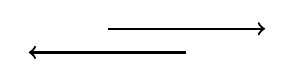
\begin{tikzpicture}=\ReadArrowType]
			\draw[->,style=thick] (2,0) -- (0,0);
			\draw[->,style=thick] (1.0,0.3) -- (3.0,0.3);
		\end{tikzpicture}
		\caption{``Outie'' overlap}
	\end{subfigure}
	\caption{The three types of overlaps.  The innie and outie overlaps are
	reverse-complement overlaps, while the normal overlap is not.  Note:
	with the normal overlap, there is a symmetric case that is not
	considered a distinct type of overlap here.}
	\label{fig:overlap_types}
\end{figure}

%\begin{enumerate}
	%\item ``Normal'' overlap
		%\begin{center}
			%\vspace{-0.5cm}
			%\begin{tikzpicture}[>=\ReadArrowType]
				%\draw[->,style=thick] (0,0) -- (2,0);
				%\draw[->,style=thick] (1.0,0.3) -- (3.0,0.3);
			%\end{tikzpicture}

			%\vspace{3mm}
			%or (symmetrically)
			%\vspace{3mm}

			%\begin{tikzpicture}[>=\ReadArrowType]
				%\draw[->,style=thick] (2,0) -- (0,0);
				%\draw[->,style=thick] (3.0,0.3) -- (1.0,0.3);
			%\end{tikzpicture}
		%\end{center}
	%\vspace{0.5cm}
	%\item ``Innie'' overlap
		%\begin{center}
			%\vspace{-0.5cm}
			%\begin{tikzpicture}[>=\ReadArrowType]
				%\draw[->,style=thick] (0,0) -- (2,0);
				%\draw[->,style=thick] (3,0.3) -- (1,0.3);
		%\end{tikzpicture} \end{center}
	%\vspace{0.5cm}
	%\item ``Outie'' overlap
		%\begin{center}
		%\vspace{-0.5cm}
		%\begin{tikzpicture}[>=\ReadArrowType]
				%\draw[->,style=thick] (2,0) -- (0,0);
				%\draw[->,style=thick] (1.0,0.3) -- (3.0,0.3);
		%\end{tikzpicture} \end{center}
%\end{enumerate}

Overlaps are important because two reads that overlap may have come from
adjacent positions on the genome.  Although due to repeats, we cannot be certain
that two overlapping reads actually came from adjacent positions, we {\em can}
say for certain that two reads that do not overlap did not come from adjacent
positions.  Regardless of this, \Figure{fig:overlap_examples} shows how two
reads that overlap potentially could be combined to form a longer sequence.

\begin{figure}
		%\begin{tikzpicture}
			%\draw (0, 0) node[anchor=left] {Read 1:}
			%\draw (0, -1) node[anchor=left] {Read 2:}
			%\draw (0, -2) node[anchor=left] {Possible genome:}
		%\end{tikzpicture}
	\centering
	\begin{subfigure}[t]{0.455\textwidth}
		1: \hspace{0.7mm}{\tt $\rightarrow$ATATAT{GCTGGTTACTT}$\rightarrow$ } \\
		2: \hspace{0.7mm}{\tt \ \ \ \ \ \ $\rightarrow${GCTGGTTACTT}TGATAGATA$\rightarrow$ } \\
		G: {\tt $\rightarrow$ATATATGCTGGTTACTTTGATAGATA$\rightarrow$}
		\caption{A normal overlap between reads (1) and (2) and the
		implied way in which the two reads could be joined together to
		form a longer sequence (G)}
	\end{subfigure}
		\hspace{0.07\textwidth}
	\begin{subfigure}[t]{0.455\textwidth}
		1: \hspace{0.7mm}{\tt $\rightarrow$ATATAT{GCTGGTTACTT}$\rightarrow$ } \\
		2: \hspace{0.7mm}{\tt \ \ \ \ \ \ $\leftarrow${CGACCAATGAA}ACTATCTAT$\leftarrow$ } \\
		G: {\tt $\rightarrow$ATATATGCTGGTTACTTTGATAGATA$\rightarrow$}
		\caption{A reverse-complement overlap between reads (1) and
		(2)--- more specifically, an ``innie'' overlap--- and the
		implied way in which the two reads could be joined together to
		form a longer sequence (G)}
	\end{subfigure}
	\caption{Examples of normal and reverse-complement overlaps}
	\label{fig:overlap_examples}
\end{figure}

\subsection{Computing overlaps}

\subsubsection{Algorithms}

Now that the idea of an exact overlap has been formalized, what we would like to
do is compute all pairwise exact overlaps of some minimum length $L$ among the
	reads that were provided as input to the assembler.  The chosen value of $L$
	must be balanced so that we find can enough overlaps to adequately cover the
	genome (small $L$ better) but still exclude most spurious overlaps (large
	$L$ better).

The naive way to compute overlaps is to consider every pair of reads in the
input, including only distinct pairs but also including the special cases of
each read paired with itself, and search for each of the types of overlaps
between the two reads in each pair.  If there are $N$ reads in the input, this
algorithm will need to consider $\frac{N^2}{2} + N$ pairs of reads. The time
spent on each read pair will depend several factors, including the minimum
overlap length $L$ and the read lengths.  But even if we could somehow spend
constant time on each read pair, this naive algorithm would be prohibitively
slow because the running time rises quadraticly with respect to the number of
reads, and there can easily be millions of reads in the input.

A number of faster algorithms for computing overlaps have been designed.  One of
the easier ones to understand is the \KeyTerm{seed-and-extend} algorithm.  It
works by indexing the reads by short subsequences of a certain length (less than
or equal to than the minimum overlap length $L$) and then only comparing reads
that actually share a subsequence.  Each of these short subsequences is called a
\KeyTerm{seed}.  Two reads may share a seed in either a forward or
reverse-complement manner.  Given two reads that share a seed, the seed can be
extended outwards in both directions to find a maximal matched region (that may
be either forward or reverse-complement) between the two reads.  Then, this
maximal matched region is compared against the definition of an overlap.  In
particular, it must be at least as long as the minimum overlap length, it must
have least 2 extreme points over the two reads, and it cannot be the prefix or
suffix of both reads if the match does not extend to the opposite end of at
least one of the reads.  If all of these conditions are met, this maximal matched
region is translated into an overlap and added to the set of overlaps if not
already present.

The running time of this seed-and-extend algorithm is
typically much faster than the naive algorithm, although it is highly dependent
on the data.  The number of distinct seeds is at worst linear with respect to
the genome length.
%of a DNA sequence and its reverse-complement is the lexicographically lesser of
%the two.  Here, we refer canonical form of each seed, because we wish to
%compare reads that share a seed in either a forward or reverse-complement
%manner.}
For each of these distinct seeds, the reads containing it are examined pairwise,
which takes quadratic time with respect to the number of reads sharing the
seed.  Since more reads will contain each seed when the reads are sampled more
densely from the genome, the running time of the seed-and-extend algorithm rises
quadratically with respect to read density.  In addition, the number of read
pairs the algorithm considers for a specific seed also rises quadratically with
the number of times that seed is repeated in the genome due to genomic repeats.
Overall, the seed-and-extend algorithm is not ideal and is still a bottleneck of
the entire assembly algorithm, despite the fact that it is much faster than the
naive algorithm (except in degenerate cases, such as a ``genome'' that is
entirely a single repeated letter).

\subsubsection{Implementation}

For this project, the seed-and-extend algorithm for computing overlaps was
implemented as the program \ProgramName{compute-overlaps}.  It takes as input a
file that contains a list of reads, as well as a parameter that specifies the
minimum overlap length $L$.  It produces as output (via a data structure
serialized to a file) all exact pairwise overlaps of minimum length $L$ among
reads in the input file, including reverse-complement overlaps and
self-overlaps.  The running time of the algorithm was discussed above.  The
memory usage is linear with respect to the total length of the reads and the
number of overlaps, which likely could be improved.

\begin{comment}
\begin{algorithm}
\caption{{\sc ComputeExactOverlapsNaive}($S$, $L$)}
\begin{algorithmic}
	%\FOR{{\bf each} distinct}
	\STATE b
\end{algorithmic}
\end{algorithm}

\newcommand{\OccVar}{\omega}
%\newcommand{\OccOne}{{\OccVar}_1}
%\newcommand{\OccTwo}{{\OccVar}_2}
\newcommand{\OccOne}{{\tt occ1}}
\newcommand{\OccTwo}{{\tt occ2}}
\newcommand{\SeedVar}{{\tt seed}}
\newcommand{\OccList}{{\tt occurrenceSet}}
\newcommand{\OverlapSet}{{\tt overlapSet}}
\newcommand{\OccMap}{{\tt occurrenceMap}}
\newcommand{\PosOne}{{\tt pos1}}
\newcommand{\PosTwo}{{\tt pos2}}
\newcommand{\Len}{{\tt len}}
\newcommand{\RightExtend}{{\tt rightExtend}}
\newcommand{\LeftExtend}{{\tt leftExtend}}
\newcommand{\ReadSet}{{\tt readSet}}
\newcommand{\minOverlapLen}{{\tt minOverlapLen}}
\newcommand{\readOneBeg}{{\tt read1Begin}}
\newcommand{\readOneEnd}{{\tt read1End}}
\newcommand{\readTwoBeg}{{\tt read2Begin}}
\newcommand{\readTwoEnd}{{\tt read2End}}
\newcommand{\numExtremePoints}{{\tt numExtremePoints}}

\begin{algorithm}
\caption{{\sc ComputeExactOverlapsSeedAndExtend}($\ReadSet$, $\minOverlapLen$)}
\begin{algorithmic}
	%\REQUIRE{$S$ is a list of DNA sequences}
	%\REQUIRE{$L$ is a positive integer that is the minimum overlap length}
	\STATE{Let $k$ be a positive integer less than or equal to
	$\minOverlapLen$.}
	\STATE{Let $\OccMap$ be a hash table that maps DNA sequences to sets of
		$k$-mer occurrences.}
	\STATE{Let $\OverlapSet$ be an empty set of overlaps.}
	\FOR{{\bf each} sequence $s \in \ReadSet$}
		\FOR{{\bf each} canonical $k$-mer $K \in r$}
			\STATE{Add the occurrence of $K$ to $\OccMap[K]$}
		\ENDFOR
	\ENDFOR
	\FOR{{\bf each} $(\SeedVar,\ \OccList) \in \OccMap$}
		\FOR{{\bf each} distinct pair of $k$-mer occurrences $\OccOne,
		\OccTwo \in \OccList$}
			\IF{the read ID of $\OccOne$ is greater than the read ID
			of $\OccTwo$}
				\STATE{Swap $\OccOne$ and $\OccTwo$}
			\ENDIF
			\IF{$\OccOne$ and $\OccTwo$ are both forward or both
			reverse-complement}
				\STATE{${\tt rc} \gets$ {\bf true}}
			\ELSE
				\STATE{${\tt rc} \gets$ {\bf false}}
			\ENDIF
			\STATE{$f \gets$ the read containing $\OccOne$}
			\STATE{$g \gets$ the read containing $\OccTwo$}
			\STATE{$\PosOne \gets$ the position within $f$ of $\OccOne$}
			\STATE{$\PosOne \gets$ the position within $g$ of $\OccTwo$}
			\STATE{$\Len \gets k$}
			\IF{${\tt rc}$}
				\STATE{$g' \gets$ the reverse complement of $g$}
				\STATE{${\tt \LeftExtend} \gets$ the number of
				additional bp to the left of the seed that
				match, comparing $f$ with $g'$}
				\STATE{${\tt \RightExtend} \gets$ the number of
				additional bp to the right of the seed that
				match, comparing $f$ with $g'$}
				\STATE{$\PosTwo \gets \PosTwo - {\tt
				\RightExtend}$}
			\ELSE
				\STATE{${\tt \LeftExtend} \gets$ the number of
				additional bp to the left of the seed that
				match, comparing $f$ with $g$}
				\STATE{${\tt \RightExtend} \gets$ the number of
				additional bp to the right of the seed that
				match, comparing $f$ with $g$}
				\STATE{$\PosTwo \gets \PosTwo - {\tt \LeftExtend}$}
			\ENDIF
			\STATE{$\PosOne \gets \PosOne - {\tt \LeftExtend}$}
			\STATE{$\Len \gets \Len + {\tt \LeftExtend} + {\tt \RightExtend}$}
			\IF{$\Len < \minOverlapLen$}
				\STATE{\bf continue}
			\ENDIF
			\STATE{$\readOneBeg \gets \PosOne$}
			\STATE{$\readOneEnd \gets \PosOne + \Len - 1$}
			\STATE{$\readTwoBeg \gets \PosTwo$}
			\STATE{$\readTwoEnd \gets \PosTwo + \Len - 1$}
			\STATE{$\numExtremePoints \gets 0$}
			\IF{$\readOneBeg = 0$}
				\STATE{$\numExtremePoints \gets \numExtremePoints + 1$}
			\ENDIF
			\IF{$\readOneEnd = {\sc Length}(f) - 1$}
				\STATE{$\numExtremePoints \gets \numExtremePoints + 1$}
			\ENDIF
			\IF{$\readTwoBeg = 0$}
				\STATE{$\numExtremePoints \gets \numExtremePoints + 1$}
			\ENDIF
			\IF{$\readTwoEnd = {\sc Length}(g) - 1$}
				\STATE{$\numExtremePoints \gets \numExtremePoints + 1$}
			\ENDIF


			%\STATE{Maximally extend the occurrence of $\SeedVar$ at
			%$\OccOne$ and $\OccTwo$ outwards in both directions}
			%\STATE{${\tt pos1} \gets$ the beginning of the maximally
			%matched region on the read containing $\OccOne$}
			%\STATE{${\tt pos2} \gets$ the beginning of the maximally
			%matched region on the read containing $\OccTwo$}
			%\STATE{${\tt plen} \gets$ the length of the maximally
			%matched region on the read containing $\OccTwo$}
		\ENDFOR
	\ENDFOR
\end{algorithmic}
\end{algorithm}
\end{comment}


\section{Building the fragment string assembly graph}

\label{sec:build_graph}

\subsection{Overview}

\label{subsec:graph_overview}

After overlaps have been computed from the reads, the next step is to construct
a graph that models how the reads can be assembled together when the overlaps
are used as evidence.  To do this, define a graph where each vertex corresponds
to a read\footnote{Actually, more than one read may map to the same vertex, as
explained in \Subsection{subsec:removing_contained_reads}.} and each edge
corresponds to an overlap.  Two vertices are connected by an edge if and only if
the corresponding reads share an overlap.  In addition, each edge is labeled
with an appropriate DNA sequence, the details of which will be explained later.

It needs to be decided whether each edge will be directed, undirected, or
something else.  To decide this, we need to consider exactly what each edge
needs to represent.  Consider three reads $f$, $g$, and $h$, that overlap as
follows:

\begin{center}
	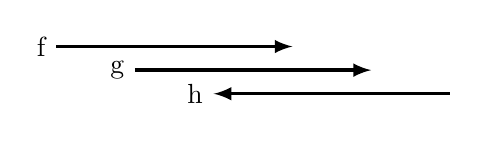
\begin{tikzpicture}[>=\ReadArrowType]
		\draw[->,style=very thick] (0,   0.6) node[anchor=east] {f} -- (3.0, 0.6);
		\draw[->,style=very thick] (1.0, 0.3) node[anchor=east] {g} -- (4.0, 0.3);
		\draw[<-,style=very thick] (2.0, 0.0) node[anchor=east] {h} -- (5.0, 0.0);
	\end{tikzpicture}
\end{center}

There are 3 overlaps, so there will be 3 edges--- one between $f$ and $g$, one
between $g$ and $h$, and one between $f$ and $h$.  As shown, the reads can be
assembled together consistently when used in the order $f,\ g,\ h$; therefore, it
must be possible to walk $f \to g \to h$ in the graph to model this assembly.
In addition, these reads could actually spell out the reverse-complement
sequence instead:

\begin{center}
	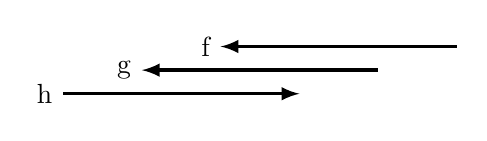
\begin{tikzpicture}[>=\ReadArrowType]
		\draw[->,style=very thick] (0,   0.0) node[anchor=east] {h} -- (3.0, 0.0);
		\draw[<-,style=very thick] (1.0, 0.3) node[anchor=east] {g} -- (4.0, 0.3);
		\draw[<-,style=very thick] (2.0, 0.6) node[anchor=east] {f} -- (5.0, 0.6);
	\end{tikzpicture}
\end{center}

Therefore, the walk $h \to g \to f$ must be allowed.  Furthermore, read $f$
directly overlaps with read $h$, so it must also be possible to walk directly $f
\to h$ or $h \to f$.

We might consider a directed graph as shown in
\Subfigure{subfig:possible_directed}, but this does not work because the graph
does not allow the reverse-complement walks such as $h \to g \to f$.

\begin{figure}
	\begin{center}
		\begin{subfigure}{0.32\textwidth}
			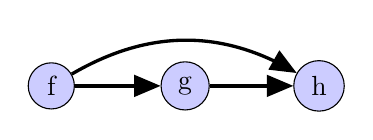
\begin{tikzpicture}[>=triangle 45]
				\tikzstyle{every node} = [circle,fill=blue!20,draw=black];
				\node (f) at (0, 0) {f};
				\node (g) at (1.7, 0) {g};
				\node (h) at (3.4, 0) {h};
				\draw[->,style=very thick] (f) edge (g);
				\draw[->,style=very thick] (g) edge (h);
				\draw[->,style=very thick,bend left] (f) edge (h);
			\end{tikzpicture}
			\caption{A possible directed \\representation of the \\string graph.}
			\label{subfig:possible_directed}
		\end{subfigure}
		\begin{subfigure}{0.32\textwidth}
			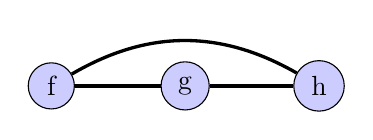
\begin{tikzpicture}[>=triangle 45]
				\tikzstyle{every node} = [circle,fill=blue!20,draw=black];
				\node (f) at (0, 0) {f};
				\node (g) at (1.7, 0) {g};
				\node (h) at (3.4, 0) {h};
				\draw[-,style=very thick] (f) edge (g);
				\draw[-,style=very thick] (g) edge (h);
				\draw[-,style=very thick,bend left] (f) edge (h);
			\end{tikzpicture}
			\caption{A possible undirected \\representation of the \\string graph.}
			\label{subfig:possible_undirected}
		\end{subfigure}
		\begin{subfigure}{0.32\textwidth}
			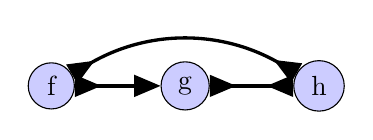
\begin{tikzpicture}[>=triangle 45]
				\tikzstyle{every node} = [circle,fill=blue!20,draw=black];
				\node (f) at (0, 0) {f};
				\node (g) at (1.7, 0) {g};
				\node (h) at (3.4, 0) {h};
				\draw[>->,style=very thick] (f) edge (g);
				\draw[>-<,style=very thick] (g) edge (h);
				\draw[>-<,style=very thick,bend left] (f) edge (h);
			\end{tikzpicture}
			\caption{A possible bidirected \\representation of the \\string graph.}
			\label{subfig:possible_bidirected}
		\end{subfigure}
		\caption{Three possibilities for constructing the string graph.  The
		bidirected construction works the best in terms of modeling the
		underlying problem.}
	\end{center}
\end{figure}

Similarly, we might consider an undirected graph as shown in
\Subfigure{subfig:possible_undirected}, but this does not work because
the graph fails to disallow walks such as $g \to h \to f$ that correspond to
assemblies that are not supported by the underlying reads.

The fundamental problem with using the directed graph is that at this stage in
the assembly, we don't know in absolute terms which strand a given read is from.
Given two reads that overlap, we can say if they are probably from the same
strand or probably from opposite strands, but we cannot say {\em in absolute
terms} which strand a given read is from.  Therefore, we must allow each read to
be used in either the forward or reverse-complement direction.  This implies
that it needs to be possible to traverse each edge in either direction, since
flipping the order of the reads in an overlap, in effect, implies that they are
reverse-complemented.  The undirected graph satisfies these requirements, but it
fails in another way: it has no guarantee that a given read is used in a
consistent way at a location within any single assembly.

The solution to all these problems is to use a new type of graph called a
\KeyTerm{bidirected graph}, shown in \Subfigure{subfig:possible_bidirected}.

\subsection{Bidirected graphs}

A \KeyTerm{bidirected graph} is a graph where a directed head is attached to both
ends of each edge.

There are 3 (or 4, ignoring symmetry) types of \KeyTerm{bidirected edges}.  They
follow directly from the different types of overlaps, as shown in
\Figure{fig:overlap_mapping}.

\begin{figure}
	\begin{center}
		\begin{tabular}{p{1cm}cccc}
			{\footnotesize Overlap} &
			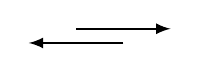
\begin{tikzpicture}[scale=0.6,>=\ReadArrowType]
					\draw[->,style=thick] (2,0) -- (0,0);
					\draw[->,style=thick] (1,0.3) -- (3,0.3);
			\end{tikzpicture}
			&
			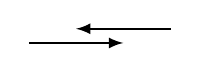
\begin{tikzpicture}[scale=0.6,>=\ReadArrowType]
					\draw[->,style=thick] (0,0) -- (2,0);
					\draw[->,style=thick] (3,0.3) -- (1,0.3);
			\end{tikzpicture}
			&
			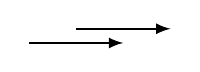
\begin{tikzpicture}[scale=0.6,>=\ReadArrowType]
					\draw[->,style=thick] (0,0) -- (2,0);
					\draw[->,style=thick] (1,0.3) -- (3,0.3);
			\end{tikzpicture}
			&
			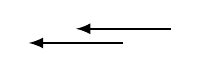
\begin{tikzpicture}[scale=0.6,>=\ReadArrowType]
					\draw[->,style=thick] (2,0) -- (0,0);
					\draw[->,style=thick] (3,0.3) -- (1,0.3);
			\end{tikzpicture}
			\\
			&$\downarrow$ & $\downarrow$& $\downarrow$& $\downarrow$ \\
			{\footnotesize Bidirected edge} &
			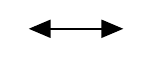
\begin{tikzpicture}[scale=0.6,>=triangle 45]
					\draw[<->,style=thick] (0,0) -- (2,0);
			\end{tikzpicture}
			&
			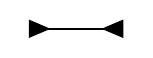
\begin{tikzpicture}[scale=0.6,>=triangle 45]
					\draw[>-<,style=thick] (0,0) -- (2,0);
			\end{tikzpicture}
			&
			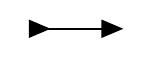
\begin{tikzpicture}[scale=0.6,>=triangle 45]
					\draw[>->,style=thick] (0,0) -- (2,0);
			\end{tikzpicture}
			&
			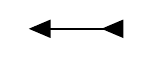
\begin{tikzpicture}[scale=0.6,>=triangle 45]
					\draw[<-<,style=thick] (0,0) -- (2,0);
			\end{tikzpicture}
		\end{tabular}
	\end{center}
	\caption{Mapping from the types of overlaps to the types of bidirected edges.}
	\label{fig:overlap_mapping}
\end{figure}

The \KeyTerm{in-degree} of a vertex $v$ in a bidirected graph is the number of
heads adjacent to $v$ that point inwards (towards $v$), while the
\KeyTerm{out-degree} of $v$ is the number of heads adjacent to $v$ that point
outwards (away from $v$).  A bidirected graph $G$ is \KeyTerm{balanced} if and
only if for every vertex in $G$ the in-degree is equal to the out-degree.

A \KeyTerm{walk} in a bidirected graph $G$ is a continuous sequence of edges in
$G$ such that if any vertex $v$ is entered through a head inwards, it is exited
through a head outwards (unless it is the end of the path), and vice versa.  An
equivalent formulation is that if we consider a possible walk in a bidirected
graph, such as the possible walk $1 \to 2 \to 3 \to 4$ in the graph shown in
\Figure{fig:bidiwalk_example}, in order to check whether the walk is valid or
not, we must consider every vertex in the possible walk except for the very
first and last vertices.  For each such vertex, we need to verify that each time
that vertex is passed through as part of a walk, the arrow heads adjacent to
that vertex that are used in the relevant part of the walk are pointed in the
same direction {\em relative to the walk}. If there are no such pairs of heads
that point towards each other or point away from each other, the walk is valid.
The red circles in \Figure{fig:bidiwalk_example} show the two pairs of heads
that need to be checked for the possible walk $1 \to 2 \to 3 \to 4$.

Note that this definition is symmetric, which implies that the reverse of a walk
in a bidirected graph is also a valid walk (e.g. the walk $4 \to 3 \to 2 \to 1$
in \Figure{fig:bidiwalk_example}).  A bidirected edge may be traversed in either
direction, possibly even during the same walk.

\begin{figure}
	\begin{center} {\small
		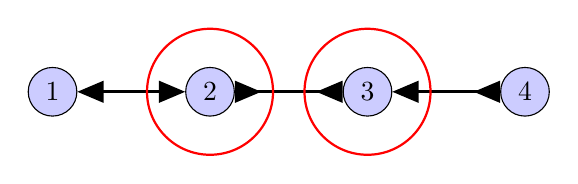
\begin{tikzpicture}[>=triangle 45]
			\tikzstyle{every node} = [circle,fill=blue!20,draw=black];
			\node (1) at (0.00, 0) {1};
			\node (2) at (2.00, 0) {2};
			\node (3) at (4.00, 0) {3};
			\node (4) at (6.00, 0) {4};
			\draw[<->,very thick] (1) edge (2);
			\draw[>-<,very thick] (2) edge (3);
			\draw[<-<,very thick] (3) edge (4);
			\draw[color=red,thick] (2.00, 0) circle (0.8);
			\draw[color=red,thick] (4.00, 0) circle (0.8);
		\end{tikzpicture}
	} \end{center}
	\caption{$1 \to 2 \to 3 \to 4$ and $4 \to 3 \to 2 \to 1$ are both valid
	walks in the bidirected graph above.  (Check circled pairs of heads to
	verify this.)}
	\label{fig:bidiwalk_example}
\end{figure}

A \KeyTerm{cycle} in a bidirected graph is a walk that begins and ends at the
same vertex in such a way that it would be a valid to trace the walk again when
the starting vertex is reached at the end of the walk.

A bidirected graph is \KeyTerm{connected} if and only if  the undirected graph
produced by replacing all bidirected edges with undirected edges is connected
(as defined for undirected graphs).  A bidirected graph is \KeyTerm{strongly
connected} if and only if it is connected and for every edge there is a cycle
containing it\cite{Medvedev2009}.

The concept of a walk in a bidirected graph maps quite nicely onto the genome
assembly problem because a walk through the bidirected string graph constructed
from a set of reads and their overlaps models a way in which the reads can be
assembled together consistently\cite{Myers2005}.  In such a walk, each read may
be used in forward or reverse-complement orientation, depending on the
direction, relative to the walk, of the adjacent arrow heads when the
corresponding vertex is passed through.

For example, consider the walk $1 \to 2 \to 3 \to 4$ in
\Figure{fig:bidigraph_mapping}.  When the walk passes through vertex 1, the
adjacent arrow head is pointed opposite the direction of the walk.  This implies
that the corresponding read is used in reverse-complement orientation.  When the
walk passes through vertex 2, the adjacent arrow heads are pointed in the
direction of the walk, which implies that the corresponding read is used in
forward orientation.  Finally, when the walk passes through vertices 3 and 4,
the adjacent arrow heads are pointed opposite the direction of the walk, which
implies that the corresponding reads are used in reverse-complement orientation.
Note that $4 \to 3 \to 2 \to 1$ is also a valid walk, which represents the way
in which the four reads could also assemble the other strand of the DNA
molecule.

\begin{figure}
	\begin{center}
		{\small
		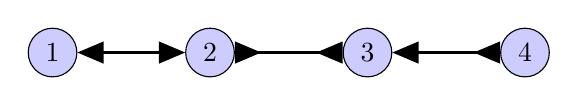
\begin{tikzpicture}[>=triangle 45]
			\tikzstyle{every node} = [circle,fill=blue!20,draw=black];
			\node (1) at (0.00, 0) {1};
			\node (2) at (2.0, 0) {2};
			\node (3) at (4.0, 0) {3};
			\node (4) at (6.0, 0) {4};
			\draw[<->,very thick] (1) edge (2);
			\draw[>-<,very thick] (2) edge (3);
			\draw[<-<,very thick] (3) edge (4);
		\end{tikzpicture} }

		\vspace{2.5mm}

		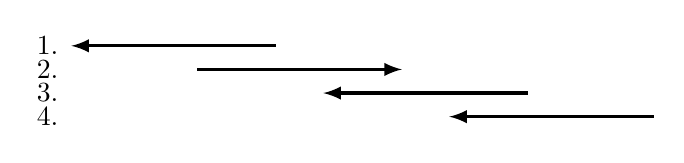
\begin{tikzpicture}[>=\ReadArrowType]
				\draw[<-,style=very thick] (0.0, 0.0) -- (2.6, 0.0);
				\draw[->,style=very thick] (1.6, -0.3) -- (4.2, -0.3);
				\draw[<-,style=very thick] (3.2, -0.6) -- (5.8, -0.6);
				\draw[<-,style=very thick] (4.8, -0.9) -- (7.4, -0.9);
				\draw (-0.3, 0.0) node {1.};
				\draw (-0.3, -0.3) node {2.};
				\draw (-0.3, -0.6) node {3.};
				\draw (-0.3, -0.9) node {4.};
		\end{tikzpicture}
	\end{center}
	\caption{A bidirected graph and the implied assembly of the
	corresponding reads}
	\label{fig:bidigraph_mapping}
\end{figure}

Earlier, a crucial point was quickly skipped over.  Each edge is supposed to be
labeled with a DNA sequence, as we are building a bidirected {\em string} graph.
However, we actually need to label each edge with two DNA sequences: one for
each direction in which the edge can be traversed.  To see this, we need to
consider exactly what it means to walk between vertices in the bidirected graph.

Consider the the string graph fragment shown in
\Subfigure{subfig:bidiedge_interp_a}.  When we walk $f \to g$, both $f$ and $g$
are used in forward orientation, as indicated by the directions of the adjacent
arrow heads.  But what this really means is that we are walking from the {\em
end} of read $f$ to the {\em end} of read $g$.  In other words, traversing the
edge in that direction is associated with the addition of the sequence after the
overlapped region in $g$, up to the end of the $g$.

If we instead walk $g \to f$, both $g$ and $f$ are used reverse-complement
orientation by walking from the {\em beginning} of read $g$ to the {\em
beginning} of read $f$.  In other words, traversing the edge in that direction
is associated with the addition of the sequence before the overlapped region in
$f$, up to the beginning of $f$, and this sequence must be reverse-complemented
because it is being used opposite its original direction.

These interpretations can be generalized to the other two types of bidirected
edges, and this is described in slightly more detail in \cite{Myers2005}.
Furthermore, these interpretations imply that the actual sequence spelled out by
a walk in the bidirected graph may include implied (non-labeled) sequence at the
start (if we start at the end of a read) and/or the end (if we end at the
beginning of a read) of the walk.

\begin{figure}
	\begin{center}
		\begin{subfigure}[b]{0.48\textwidth}
			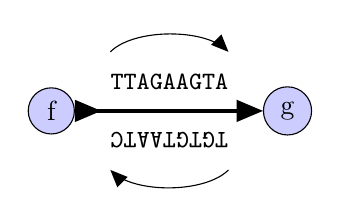
\begin{tikzpicture}[>=triangle 45,scale=1.5]
				\node[circle,fill=blue!20,draw=black] (f) at (0, 0) {f};
				\node[circle,fill=blue!20,draw=black] (g) at (2.0, 0) {g};
				\draw[>->,style=very thick] (f) edge (g);
				\draw (1.00, 0.1) node[anchor=south] {\small \tt TTAGAAGTA};
				\draw (1.00, -0.1) node[anchor=north] {
						\rotatebox{180}{\small \tt
						TGTGTAATC}};
				\draw[->] (0.5, 0.5) ..
					controls (0.7, 0.7) and (1.3, 0.7) ..
					(1.5, 0.5);
				\draw[->] (1.5, -0.5) ..
					controls (1.3, -0.7) and (0.7, -0.7) ..
					(0.5, -0.5);
			\end{tikzpicture}
			\caption{A bidirected string graph fragment}
			\label{subfig:bidiedge_interp_a}
		\end{subfigure}
		\begin{subfigure}[b]{0.48\textwidth}
			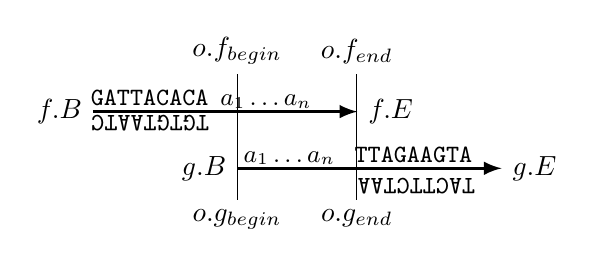
\begin{tikzpicture}[>=\ReadArrowType,scale=0.8]
				\draw[->,very thick] (-0.2, 0) node[anchor=east] {$f.B$}
						-> (4, 0) node[anchor=west] {$f.E$};
				\draw[->,very thick] (2.09, -0.9) node[anchor=east] {$g.B$}
						-> (6.29, -0.9) node[anchor=west] {$g.E$};

				\draw (-0.2, -0.1) node[anchor=south west]
					{\hspace*{-1.5mm}{\small \tt
						%GATTACACAGTGTAGTT
						GATTACACA\hspace*{1.5mm}$a_1 \dots a_n$
					}};

				\draw (-0.2, 0.1) node[anchor=north west]
					{\hspace*{-2.6mm}
						\rotatebox{180}{{\small \tt TGTGTAATC}}};

				\draw (2.09, -1.0) node[anchor=south west]
					{\hspace*{-1.4mm}{\small \tt
						%GTGTAGTTTTAGAAGTA
						\hspace*{0.1cm}$a_1 \dots a_n$\hspace*{0.25cm}TTAGAAGTA
					}};

				\draw (2.09, -0.9) node[anchor=north west]
					{\hspace*{12.88mm}
						\rotatebox{180}{{\small \tt TACTTCTAA}}};

				\draw (2.09, -1.4) node[anchor=north] {$o.g_{begin}$}
						-- (2.09, 0.6) node[anchor=south] {$o.f_{begin}$};
				\draw (3.99, -1.4) node[anchor=north] {$o.g_{end}$}
						-- (3.99, 0.6) node[anchor=south] {$o.f_{end}$};
			\end{tikzpicture}
			\caption{The corresponding overlap (labeled)}
			\label{subfig:bidiedge_interp_b}
		\end{subfigure}
	\end{center}

	\begin{subfigure}{1.00\textwidth}
		\begin{center}
			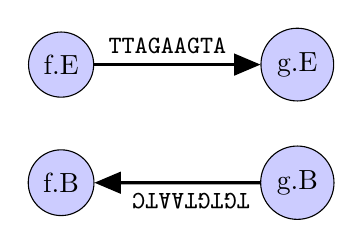
\begin{tikzpicture}[>=triangle 45,scale=1.5]
				\node[circle,fill=blue!20,draw=black] (fE) at (0, 0) {f.E};
				\node[circle,fill=blue!20,draw=black] (gE) at (2.0, 0) {g.E};

				\node[circle,fill=blue!20,draw=black] (fB) at (0, -1) {f.B};
				\node[circle,fill=blue!20,draw=black] (gB) at (2.0, -1) {g.B};

				\draw[->,style=very thick] (fE) edge (gE);
				\draw[->,style=very thick] (gB) edge (fB);
				\draw (0.90, 0.01) node[anchor=south] {\small \tt TTAGAAGTA};
				\draw (1.10, -1.01) node[anchor=north] {
						\rotatebox{180}{\small \tt
						TGTGTAATC}};
			\end{tikzpicture}
		\end{center}
		\caption{The corresponding directed string graph fragment}
		\label{subfig:bidiedge_interp_c}
	\end{subfigure}

	\vspace{1.0cm}

	\begin{subfigure}{1.00\textwidth}
		\begin{center}
			\begin{tabular}{c|c}
				walk & interpretation \\ \hline
				$f \to g$ & $f.E \to g.E$ with sequence $g[o.g_{end} + 1 \dots ${\tt
				length}$(g)]$ \\
				$g \to f$ & $g.B \to f.B$ with sequence $f[o.g_{begin} - 1 \dots 0]$ \\
			\end{tabular}
		\end{center}
		\caption{Interpretation of each walk on the bidirected graph fragment}
	\end{subfigure}
	\caption{Full interpetation of an edge in a bidirected string graph}
	\label{fig:bidiedge_interp}
\end{figure}

\subsection{An equivalent directed graph model}

\label{subsec:directed}

In \Subsection{subsec:graph_overview}, the possibility of using a directed graph
to model the assembly of the reads was rejected because it did not take into
account the double-strandedness of DNA.  However, \Figure{fig:bidiedge_interp}
suggests an alternate construction of the graph that does indeed use directed
edges.  Instead of having each vertex be a read, have each vertex be an end of a
read.  The advantage to this approach is that the problem can be expressed using
a directed graph instead a bidirected graph, which can be helpful for the
implementation.  The disadvantage is that there are two completely separate
vertices for each read.

\subsection{Removing contained reads}

\label{subsec:removing_contained_reads}

Earlier, the definition of a \KeyTerm{contained read} was provided.  Contained
reads need not be included in the graph because there will always be a walk that
spells the sequence of each contained read.  In other words, contained reads
provide redundant information because the sequence of any given contained read
is already spelled out by an uncontained read.

Therefore, prior to mapping the reads to vertices and overlaps to edges, we can
examine the overlaps to identify contained reads, and include in the initial
construction of the bidirected string graph neither the contained reads nor any
overlaps involving a contained read.

This implies that a vertex in the bidirected string graph may actually
correspond to more than one read.

The contained reads cannot be completely discarded because they are needed for a
later step (see \Subsection{subsec:mapping_contained_reads}).

\subsection{Implementation of assembly graph construction}

As described in \Subsection{subsec:removing_contained_reads}, before the
assembly graph is even built, contained reads need to be removed.  This is
implemented by the program \ProgramName{remove-contained-reads}.  It takes as
input two files: the set of reads and the set of overlaps that were computed
from them, and produces as output three files: the set of uncontained reads, the
set of overlaps excluding those that involve contained reads, and an array that
maps from the original read indices to the new read indices.

Building the graph is implemented by either the program
\ProgramName{build-bidirected-string-graph} or the program
\ProgramName{build-directed-string-graph}, the latter of which builds the
directed equivalent to the bidirected graph described in
\Subsection{subsec:directed}.  Both programs take as input two files: the set of
uncontained reads and their overlaps, and produce as output the bidirected or
directed graph, serialized to a file.  As should be expected from what was
described earlier, \ProgramName{build-bidirected-string-graph} will add one
vertex for each read and add a bidirected edge for each overlap, while
\ProgramName{build-directed-string-graph} will add two vertices for each read
and add two directed edges for each overlap.

The string graphs are stored in a binary format.  An additional program,
\ProgramName{print-string-graph}, was implemented that can print a string graph
in plain-text format, print a string graph in the DOT language for input to the
graph-drawing software {\it GraphViz}\cite{GraphVizPublication}, or print some
other information about a string graph.

Furthermore, programs \ProgramName{bidigraph-to-digraph} and
\ProgramName{digraph-to-bidigraph} were implemented to convert between the
bidirected and directed representations of the string graph.

A program \ProgramName{extract-edge-seqs} was implemented to extract the
sequences that the edges are labeled with, as this can be done to produce a
preliminary assembly (especially after the graph simplifications that are about
to be described).

\section{Simplifying the assembly graph}

\subsection{Transitive reduction}

Before trying to find walks through the string graph, it is very helpful to
simplify the graph is much as possible.  Very commonly, given three adjacent
reads $f$, $g$, and $h$, $f$ will overlap $h$ as well as $g$.  This is redundant
because we can, equivalently, walk $f \to g \to h$ rather than directly walking
from $f \to h$.  \Figure{fig:transitive} shows an example of this.

\begin{figure}
	\begin{center}
		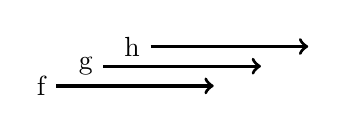
\begin{tikzpicture}
			\draw[->,style=very thick] (0,0) node[anchor=east] {f} -- (2,0);
			\draw[->,style=very thick] (0.6,0.25) node[anchor=east] {g} -- (2.6,0.25);
			\draw[->,style=very thick] (1.2,0.5) node[anchor=east] {h} -- (3.2,0.5);
		\end{tikzpicture}
		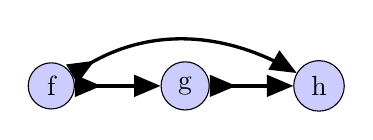
\begin{tikzpicture}[>=triangle 45]
			\tikzstyle{every node} = [circle,fill=blue!20,draw=black];
			\node (f) at (0, 0) {f};
			\node (g) at (1.7, 0) {g};
			\node (h) at (3.4, 0) {h};
			\draw[>->,style=very thick] (f) edge (g);
			\draw[>->,style=very thick] (g) edge (h);
			\draw[>->,style=very thick,bend left] (f) edge (h);
		\end{tikzpicture}
	\end{center}
	\caption{Three overlapping reads $f$, $g$, and $h$, and the corresponding
	bidirected graph.  The edge between $f$ and $h$ is transitive and is removed
	by transitive reduction.}
	\label{fig:transitive}
\end{figure}

Walks visiting more vertices are preferred because they are supported by more
reads and the overlaps tend to be longer.  So, we would like to throw away
\BidirectedEdgeForward{$f$}{$h$}, which is a \KeyTerm{transitive edge}, but keep
\BidirectedEdgeForward{$f$}{$g$} and \BidirectedEdgeForward{$g$}{$h$}.

To remove these redundant edges, \KeyTerm{transitive reduction} is performed on
the bidirected string graph.

\Algorithm{alg:transitive_reduction} provides pseudocode for a transitive
reduction algorithm similar to that described in \cite{Myers2005}.  Essentially,
the algorithm is to through each vertex $v$ and examine vertices up to 2 edges
away from $v$ to identify all transitive edges leaving $v$.  These edges are
then marked for removal, and they are removed after all vertices in the graph
have been considered.  Some optimizations are possible; for example, the lengths
of the sequences the edges are labeled with can be taken into account to allow
terminating the search of $v$'s neighborhood before all possible walks of length
2 starting at $v$ have been considered.

Transitive reduction can be performed on either the bidirected or directed
representations of the string graph, although for simplicity
\Algorithm{alg:transitive_reduction} implies the directed representation.

\begin{algorithm}
	\caption{{\sc TransitiveReduction}($G$)}
	{\footnotesize
		\begin{algorithmic}
			\FOR{{\bf each} vertex $v \in G$}
				\STATE{Mark all neighbors of $v$ as {\tt INPLAY}}
				\STATE{Set {\tt longest} $\gets$ length of the longest edge leaving $v$}
				\FOR{{\bf each} edge $v \to w$ in order of length}
					\FOR{{\bf each} edge $w \to x$ in order of length}
						\IF{$x$ is not marked {\tt INPLAY}}
							\STATE{\bf continue}
						\ENDIF
						\IF{$len(v \to w) + len(w \to x) > $ {\tt longest}}
							\STATE{\bf break}
						\ENDIF
						\STATE{Mark $x$ as {\tt ELIMINATED}}
					\ENDFOR
				\ENDFOR
				\STATE{Mark as transitive all edges $v \to x$ where $x$ is marked {\tt ELIMINATED}}
			\ENDFOR
			\STATE{Eliminate all edges marked transitive}
		\end{algorithmic}
	}
	\label{alg:transitive_reduction}
\end{algorithm}

Transitive reduction on a string graph is implemented as the program
\ProgramName{transitive-reduction}.  It takes as input a file containing a
string graph and produces as output a file containing the transitively reduced
string graph.

\subsection{Collapsing unbranched paths}

After transitive reduction, a non-repetitive region of the genome will typically
be represented in the string graph by a chain of vertices that is part of a
valid walk and consists entirely of vertices with in-degree 1 and out-degree 1.
This is referred to as an \KeyTerm{unbranched path}, and it contains one or more
\KeyTerm{inner vertices}.  An unbranched path can be collapsed by removing the
inner vertices and replacing them by a single edge that covers the entire path.
This replacement edge is labeled with the concatenation of the sequences that
the edges are labeled with.  In the bidirected case, this concatenation must be
done for both directions in which the unbranched path might have been traversed.
\Figure{fig:collapse_unbranched_paths} shows an example of how a short
unbranched path can be collapsed.

Collapsing unbranched paths is implemented as the program
\ProgramName{collapse-unbranched-paths}.  It takes as input a file containing a
string graph and produces as output a file containing the string graph with
unbranched paths collapsed.  Vertices are currently re-numbered; so, for
example, vertex 10 after collapsing unbranched paths does not necessarily refer
to the 10th read in the list of uncontained reads from which the graph was
constructed.

\begin{figure}
	\begin{center}
		{\small
		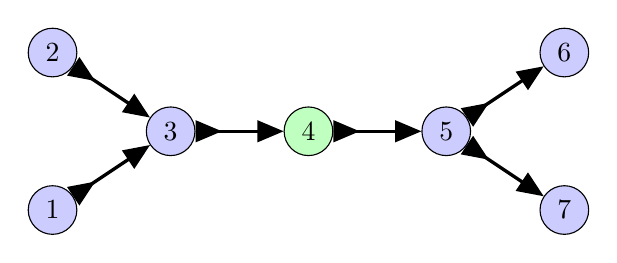
\begin{tikzpicture}[>=triangle 45]
			\tikzstyle{every node} = [circle,fill=blue!20,draw=black];
			\node (1) at (0.0, -1) {1};
			\node (2) at (0.0, 1) {2};
			\node (3) at (1.5, 0) {3};
			\node[fill=green!25] (4) at (3.25, 0) {4};
			\node (5) at (5.0, 0) {5};
			\node (6) at (6.5, 1) {6};
			\node (7) at (6.5, -1) {7};
			\draw[>->,very thick] (1) edge (3);
			\draw[>->,very thick] (2) edge (3);
			\draw[>->,very thick] (3) edge (4);
			\draw[>->,very thick] (4) edge (5);
			\draw[>->,very thick] (5) edge (6);
			\draw[>->,very thick] (5) edge (7);
		\end{tikzpicture}
		}

	becomes:

		{\small
		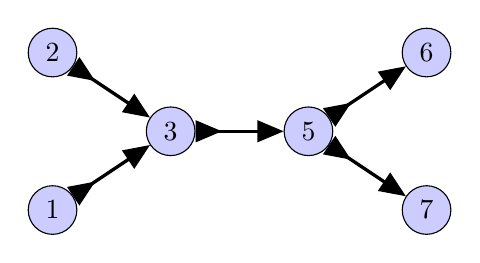
\begin{tikzpicture}[>=triangle 45]
			\tikzstyle{every node} = [circle,fill=blue!20,draw=black];
			\node (1) at (0.0, -1) {1};
			\node (2) at (0.0, 1) {2};
			\node (3) at (1.5, 0) {3};
			\node (5) at (3.25, 0) {5};
			\node (6) at (4.75, 1) {6};
			\node (7) at (4.75, -1) {7};
			\draw[>->,very thick] (1) edge (3);
			\draw[>->,very thick] (2) edge (3);
			\draw[>->,very thick] (3) edge (5);
			\draw[>->,very thick] (5) edge (6);
			\draw[>->,very thick] (5) edge (7);
		\end{tikzpicture}
		}
	\end{center}
	\caption{Vertex 4 an \KeyTerm{inner vertex} that is part of an unbranched
	path that can be collapsed.  Edge labels are not shown.}
	\label{fig:collapse_unbranched_paths}
\end{figure}

\section{Examples of assembly graph construction and simplification}

At this point, the assembler has been given a set of reads, has computed exact
overlaps from them, has removed contained reads and all overlaps involving them,
has built a bidirected string graph that models the ways in which the reads can
be assembled together when the overlaps are used as evidence, and has simplified
this graph through transitive reduction and collapsing unbranched paths.
Usually, the graph at this point will be much simpler than the original graph,
although it may still be very complicated, depending on the genome and the data.

\subsection{Random genome}

A completely random genome is very unlikely to have repeats of significant
length compared to the minimum overlap length.  In this case, transitive
reduction is expected to leave the entire graph as a single unbranched path,
provided the original genome was a single, non-circular string and every base
pair of it was included in at least one read.  Then, collapsing unbranched paths
will collapse the entire bidirected graph into two vertices connected by a
single edge.  Finding a walk through the edges of this graph is trivial and will
produce an assembly of the entire genome.  \Figure{fig:random_example} shows the
bidirected string graph that might result from such a genome and data.

If we still assume a genome with no repeats of length greater than the overlap
length, but relax the assumption that the genome is a single, non-circular
string from which every base pair was included in a read, the graph will instead
reduce and collapse to a set of components.  Components corresponding to
non-circular sequence will contain two vertices with an edge between, while
components corresponding to circular sequence will contain one vertex with an
edge connecting it to itself (a loop).  In this case (and as will be elaborated
on later), finding a walk through the bidirected string graph must be
generalized to allow walking each component separately; but again for this
particular case of a random genome, each such walk is still trivial, and the
assembly will be optimal as long as the assembler does not decide to traverse
any of the loops more than one time (this will also be elaborated on more
later), since there are no repeats of substantial length in a hypothetical
random genome.

\begin{figure}
	\begin{center}
		\vspace{1cm}
		\begin{tikzpicture}
			{\small
			\begin{tikzpicture}[>=triangle 45]
				\node[circle,fill=blue!20,draw=black] (A) at (0.0, 0) {A};
				\node[circle,fill=blue!20,draw=black] (B) at (3.0, 0) {B};
				\draw[>->,very thick] (A) edge node[anchor=north] {4639100} (B);
			\end{tikzpicture} }
		\end{tikzpicture}
		\caption{
			Bidirected string graph for reads uniformly sampled from a 4.6 Mbp
			random genome after transitive reduction and path collapsing.  (Edge
			labeled with length of sequence, with the length being the same in both
			directions)}
		\label{fig:random_example}
	\end{center}
\end{figure}

\subsection{Real genome}

Real genomes are not random, and they contain far more repeats than would be
expected purely by chance.\footnote{Biologically, repeats can occur for a number
of reasons, such as gene duplications.} \Figure{fig:E_coli} shows an example of
the simplified bidirected string graph for a real genome.  It is apparent that
even when using perfect, fairly long reads that cover the entire genome, the
repeats in the genome cause branches to appear in the graph when the repeats are
too long to be resolved by the reads at this stage in the assembly.

\begin{figure}
	\begin{center}
		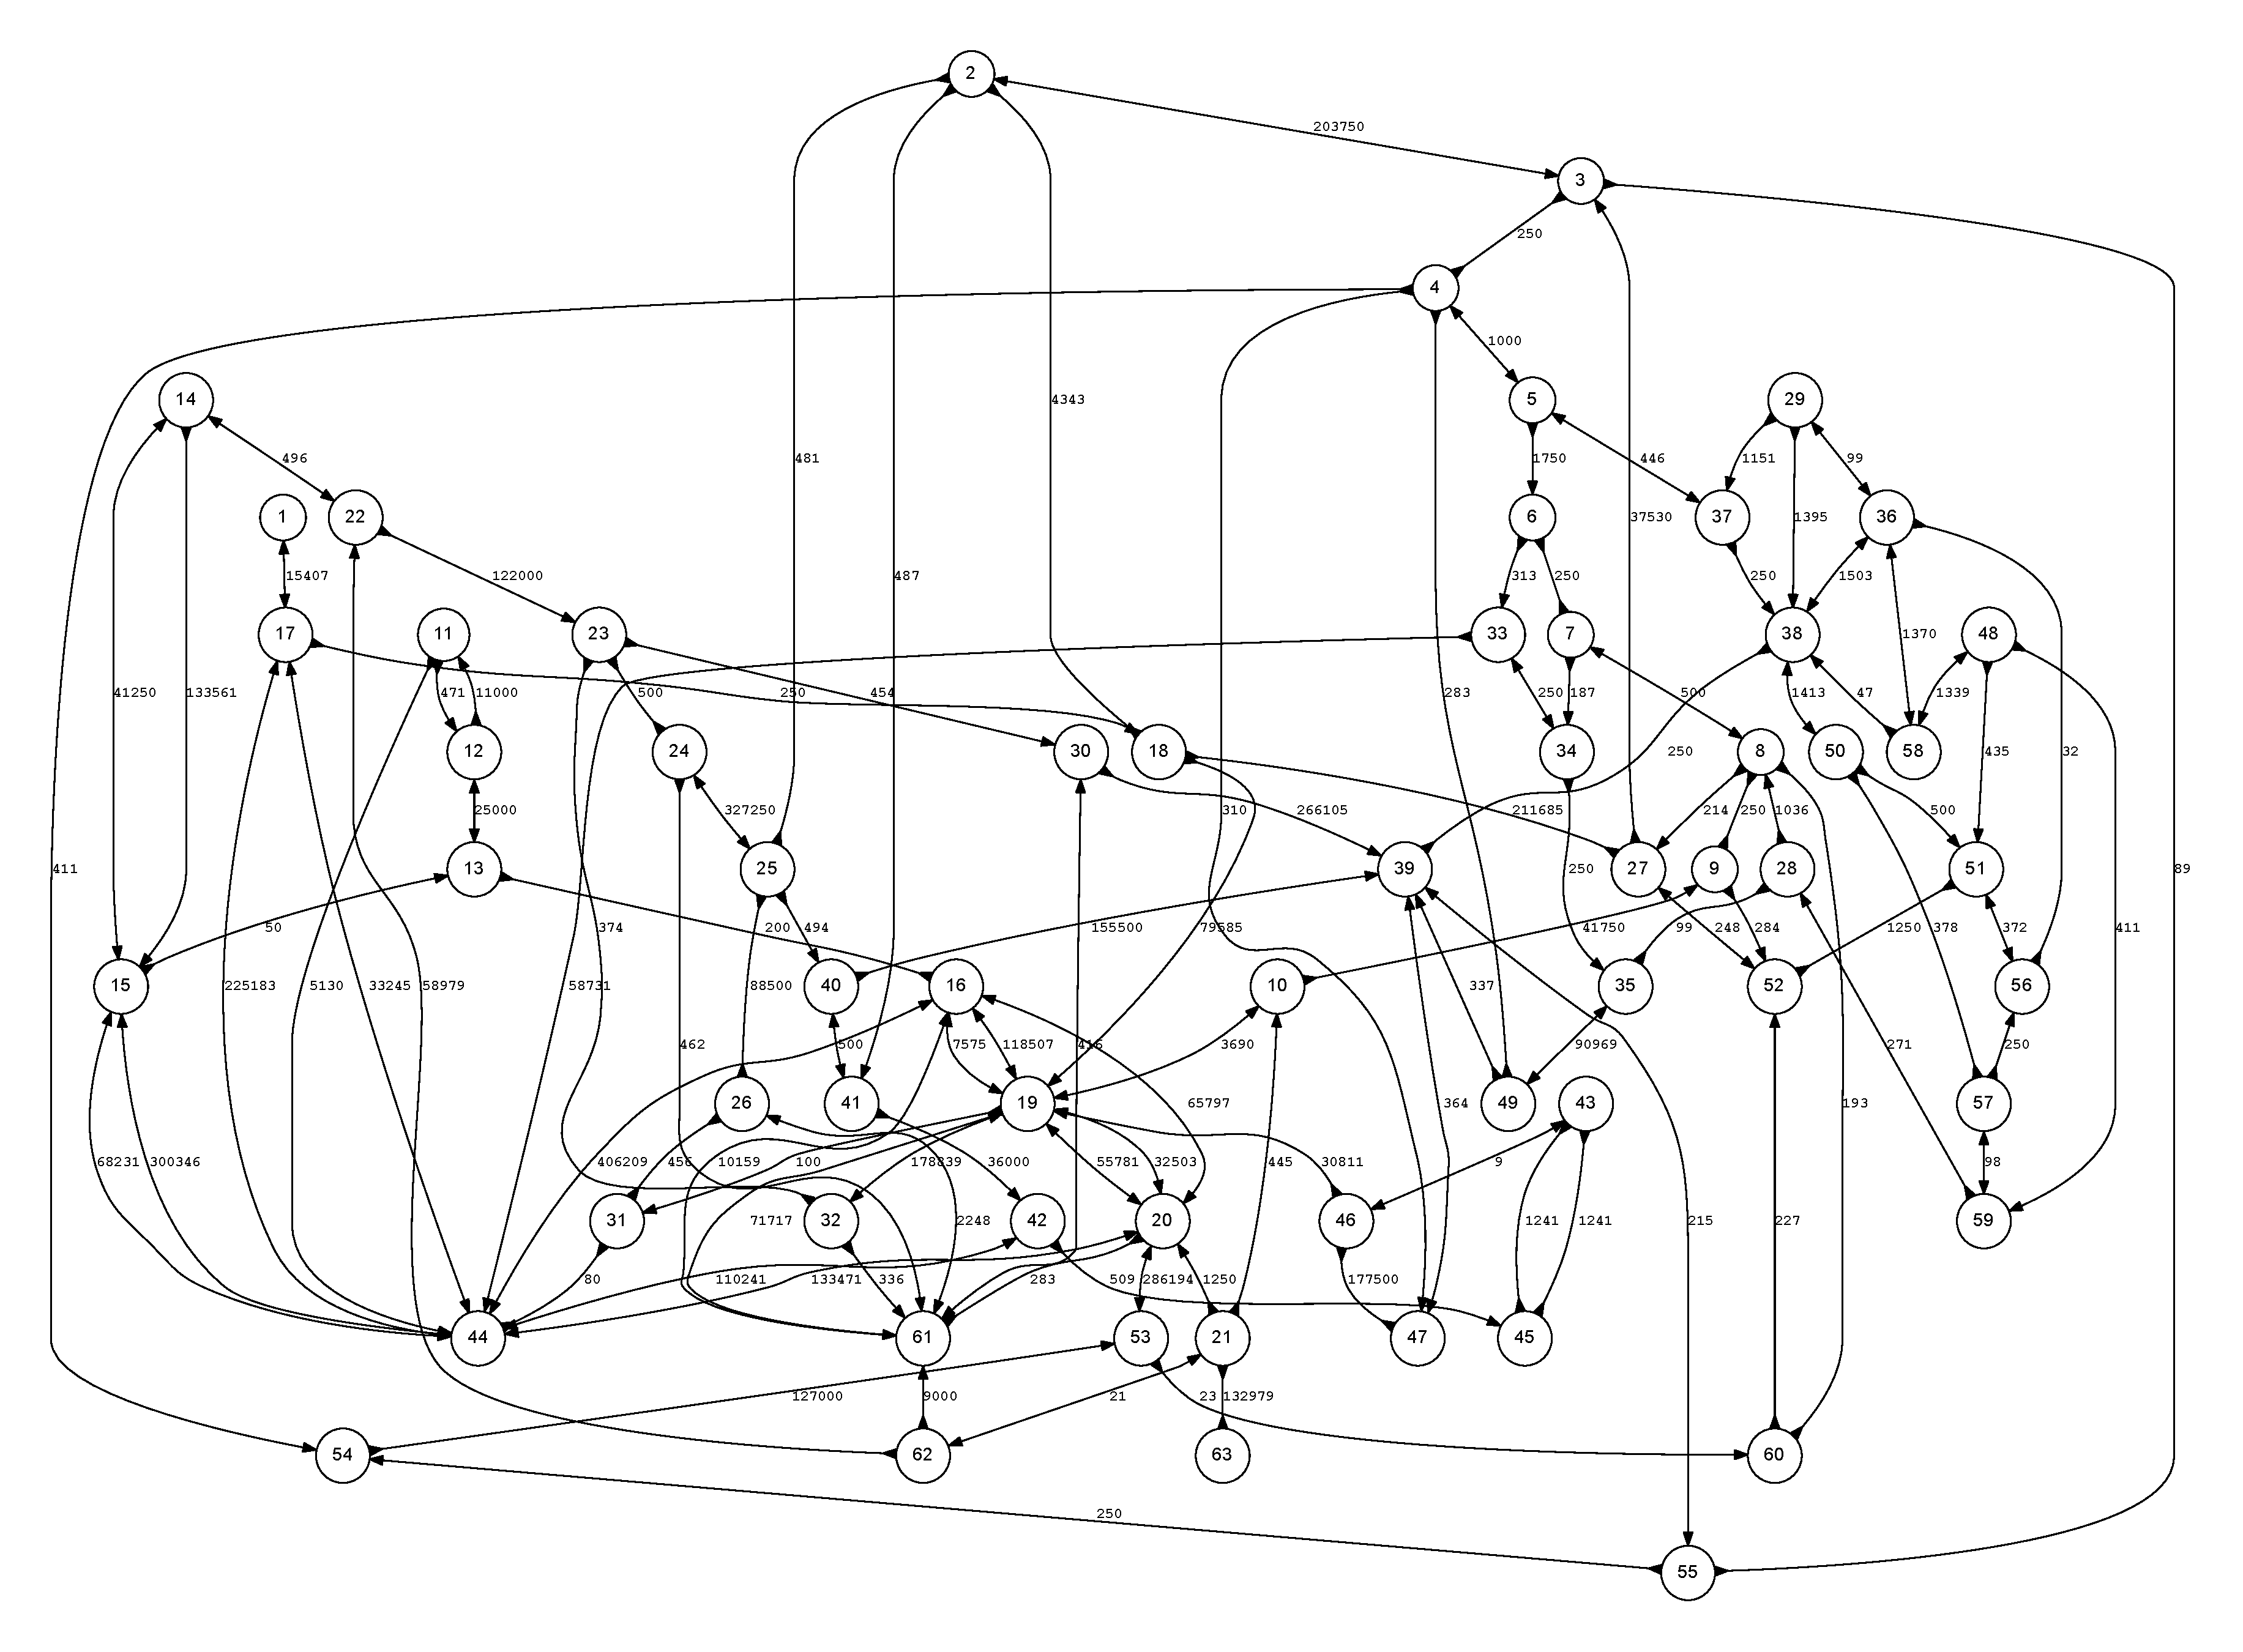
\includegraphics[width=1.0\textwidth]{E_coli.pdf}
		\caption{Transitively-reduced, collapsed bidirected string graph for
		1000 bp perfect reads uniformly sampled every 100 bp from random strands
		of the non-circular version of the 4,639,675 bp genome of {\it E. coli}
		(a common bacterium) using a minimum overlap length of 250 bp.  This
		graph was produced by the code that has been discussed, but the actual
		drawing of the picture was done by {\it
		GraphViz}\cite{GraphVizPublication}.  The 46,387 reads
		that were provided as input to the assembler were generated by a Perl
		script.  The bottleneck of the algorithm up to this point is
		\ProgramName{compute-overlaps}, which took about 10 minutes and used a
		maximum of about 1 GiB of memory to find all 336,227 overlaps from these
		reads, seeding on 128-mers.  The running time and memory usage of
		\ProgramName{compute-overlaps} would need to improved further to handle
		larger genomes.}
		\label{fig:E_coli}
	\end{center}
\end{figure}

\subsection{Small step-by-step example}

\section{Producing the final assembly}

\label{sec:final}

\subsection{Overview}

As \Figure{fig:E_coli} shows, the bidirected string graph may still be very
complicated even after transitive reduction and traversal.  In even worse
examples, the graph could easily have thousands of vertices and edges, and it
may not even be connected.  Therefore, we need to figure out how to walk through
the graph to produce the best assembly.

An \KeyTerm{Eulerian path in a bidirected graph} is a walk that traverses each
bidirected edge exactly one time in either direction.  Suppose we could find an
Eulerian path in the bidirected string graph.  Then this path would correspond
to an assembly that accounts for every overlap and therefore would be a valid
assembly of the original reads.  Furthermore, such a path may allow for vertices
to be used for than one time in the assembly to allow for genomic repeats, which
would not be true if we found a Hamiltonian path instead.\footnote{A Hamiltonian
path is also inappropriate here because unbranched paths have been collapsed
into single edges, which {\em must} be included in the assembly if the reads
corresponding to the inner vertices are to take part in the assembly.
Furthermore, keep in mind that there is not a one-for-one correspondence between
vertices and reads because contained reads were removed (see
\Subsection{subsec:removing_contained_reads}).}

However, there are multiple problems with the Eulerian path approach.  First,
the graph may not be Eulerian.  This could happen if the graph is not balanced.
This implies we really would need to solve the bidirected equivalent of the
Chinese Postman Problem instead.\footnote{The Chinese Postman problem on a
bidirected graph is formalized in \cite{Medvedev2009}.}  Even then, the graph
may not be fully connected, which would require that the final walk take the
form of multiple discontinuous walks.  An equally severe problem is that some
overlaps may be spurious, meaning that the two overlapping reads do not actually
form a valid genomic sequence when combined.  Spurious overlaps can be caused by
genomic repeats.  Therefore, we need to allow for the possibility that an edge
in the bidirected graph can be omitted from the walk if it seems like a good
idea to do so.

The way these problems can be solved is to (1) place a lower bound and an upper
bound on the number of times each edge may be traversed, then (2) formulate and
solve a minimum-cost circulation problem that finds the minimum total traversal
count of edges in the graph in order for every vertex to be balanced (i.e. have
the same in-degree as out-degree), then (3) find a generalized Eulerian tour
through the bidirected graph, traversing each edge the exact number of times
that was calculated in (2) and also allowing for the tour be discontinuous.

\subsection{Calculating the A-statistic}

\label{subsec:a_statistics}

We would like to use hints from the original data to restrict the number of
times each bidirected edge may be traversed.  This can be done using a
calculation called the \KeyTerm{A-statistic}, or \KeyTerm{arrival-rate
statistic}, which is the logarithm of the probability that an edge represents
unique sequence rather than duplicate sequence \cite{Myers2005}.  The A-statistic
$A(e)$ of an edge $e$ in a bidirected string graph is:

\[ A(e) = \frac{n}{G} \Delta - \ln{2} \cdot {k} \]

where $n$ is the total number of reads, $G$ is the estimated genome length,
$\Delta$ is the length of the edge in bp, and $k$ is the number of reads that
support that edge.  To more precise, $k$ is the number of inner vertices in the
unbranched path corresponding to $e$ before the unbranched paths were collapsed
\cite{Myers2005}.

Edges with sufficiently high A-statistic are very likely to be single-copy edges
and therefore should be traversed exactly one time.  The remaining edges may be
traversed any number of times (with the exact number being determined during the
minimum-cost circulation calculation), except for edges that originally were
associated with one or more inner vertices, in which case we require the edge be
traversed at least one time so that the reads corresponding to the inner
vertices are used in the reconstruction of the genome.  This is needed because
in the absence of foreign DNA, every read was presumably sampled from the
genome.

However, $G$, the estimated genome length, is actually unknown, so it must be
estimated first.  It can be estimated by producing a ``bootstrap'' genome length
by adding up the lengths of the sequences on every edge in both directions and
dividing by 2, then calculating the A-statistics using this bootstrap genome
length and identifying edges that are probably single-copy.  The A-statistics
can then be re-estimated over just these single-copy edges in order to refine
the genome length further before calculating the final A-statistic on all the
edges.  This procedure was outlined in \cite{Myers2005}.

The calculation of the A-statistic on each edge in the bidirected string graph,
including the genome length bootstrapping algorithm, is implemented by the
program {\tt calculate-A-statistics}.

\subsection{Mapping contained reads}

Because contained reads and their overlaps were removed before constructing the
assembly graph (see \Subsection{subsec:removing_contained_reads}), the
calculation of the A-statistic as described above is flawed because contained
reads need to be counted.  This is especially a problem for high copy-number
regions because those regions are likely to generate many contained reads.
Therefore, we need to map the contained reads into the graph before calculating
the A-statistics.

A contained read may easily be mapped to the vertex corresponding to a read that
contains it, but this is not sufficient because the A-statistic is calculated
over the edges, not the vertices.  Instead, we need to map each end of each the
contained read to the edge, or in general the set of edges, that contains it.

The algorithm for doing so is outlined in \cite{Myers2005} and was implemented
by the program \ProgramName{map-contained-reads}, which runs before
\ProgramName{collapse-unbranched-paths}.  Briefly, for each contained read $r$
the algorithm identifies the uncontained read $R$ that contains $r$ and has the
shortest distance from the end of $r$ to the end of $R$ (the shortest
\KeyTerm{overhang}).  This is done for each of the two directions.  The edges in
the graph starting at the vertex corresponding to that end of $R$ are then
walked backwards for the length of the overhang to find the set of edges $S$ to
which the corresponding edge of $r$ may map, and each edge in $S$ is marked as
containing $\frac{1}{|S|}$ extra inner vertices.  This mapping, therefore, makes
it possible to account for contained reads when calculating the A-statistic.

\label{subsec:mapping_contained_reads}

\subsection{Minimum-cost circulation}

Formally, a minimum-cost circulation problem on a directed graph takes as input
for each edge $e$ an lower bound $l(e) \ge 0$ and an upper bound $u(e) \ge 0$ on
flow and a cost per unit flow $v(e)$, and for each vertex $v$ a supply
(positive) or demand (negative) $b(v)$ for flow.  It produces as output a flow
$x(e)$ on each edge $e$ such that $\sum_e v(e)x(e)$ is minimized subject to
$x(e) \in [l(e), u(e)]$ and $\sum_{u \to v}x(u \to v) + b(v) = \sum_{v \to w}
x(v \to w)$ \cite{Myers2005}.  In the minimum-cost circulation problem, as
opposed to less general network flow problems, no nodes are treated specially as
sources or sinks; instead, flow must be balanced at every node $v$, but only
after taking into account the supply or demand $b(v)$ at that node.

The A-statistic calculation on each edge $e$, as described in
\Subsection{subsec:a_statistics}, allows us to assign a lower bound $l(e)$ and
an upper bound $u(e)$ on the traversal count for that edge.  Note that $u(e)$
may be $\infty$, as these bounds are very approximate.  We also have $b(v) = 0$
for all $v$, because the flow at every vertex must be balanced; this corresponds
to the walk entering each vertex the same number of times that it is exited,
making the graph as a whole be balanced.

%It produces as output a flow
%$x(e)$ on each edge $e$ such that $\sum_e v(e)x(e)$ is minimized subject to
%$x(e) \in [0, c(e)]$ and $\sum_{u \to v}x(u \to v) + b(v) = \sum_{v \to w} x(v
%\to w)$.\cite{Myers2005}.

%We can roughly map our problem onto this definition assigning $c(e) = 0$ when
%$e$ is definitely single-copy and $c(e) = \infty$ otherwise, $b(v)$ the sum
%of the lower bounds on the traversal counts of all bidirected edges incident to
%$v$ with an inward head minus the sum of the lower bounds on the traversal
%counts of all edges incident to $v$ with an outward head, and $v(e) = 1$.  The
%resulting traversal count $t(e)$ for a bidirected edge $e$ is then the lower
%bound on the traversal count for that edge plus $x(e)$, the traversal count
%assigned in the network flow calculation.  The traversal count $t(e)$ represents
%the total number of times the edge may be traversed in a given assembly,
%counting traversals in both directions.

There are still two serious problems with this circulation formulation that need
to be addressed.  First, we actually have a bidirected graph, not a directed
graph.\footnote{The fact that this circulation problem actually needs to be
formulated and solved on a bidirected graph is addressed in \cite{Medvedev2009},
but not in \cite{Myers2005}, even though the latter introduced the overall
fragment string graph algorithm.}

but is a.  We have a
bidirected graph, not a directed graph, so it cannot be trivially mapped to a
directed network flow problem.  A possible workaround for this is to solve
directed flow on the directed equivalent to the bidirected graph, described in
\Subsection{subsec:directed}.  The calculated traversal counts for a directed
edge $e$ between, for example, two vertices $f.E \to g.E$ is not guaranteed to
be the same as the calculated traversal count for the edge that corresponds to
the other direction of the implied bidirected edge, which would be $g.B \to f.B$
in this example.  However, we can take the average of the two counts and use
this as the traversal count for the corresponding bidirected edge, and this 

%vertices $f.X$ and $g.X

\subsection{Generalized Eulerian path}

\section{Implementation}

The implementation of the fragment string graph algorithm that was done for this
project is a set of C++ programs that iteratively transform the data on-disk
into the final assembly.  Each program takes as input one or more files as well
as zero or more other command-line arguments and produces as output one or more
files.  Each file contains data such as a list of reads, a list of overlaps, or
a graph.  Internally to the assembler pipeline, data is stored in binary form.
\Figure{fig:impl_graph} shows how the data flows through the main stages of the
assembler.

The input to the assembler is one or more files in plain-text form that each
contain a list of reads.  The final output of the assembler will eventually be a
file in plain-text format that gives the list of assembled contigs.  Currently,
the final stages of the algorithm (\Section{sec:final}, except for the
calculation of the A-statistics) have not been implemented as of the end of the
semester of Fall 2012.

\begin{figure}
	\begin{center}
		\includegraphics[width=0.7\textwidth]{programs.pdf}
	\end{center}
	\caption{The flow of data through the assembly pipeline.  Each node is a
	program, each arrow represents the output of a program being used as input
	in another program.  Yellow programs have not yet been implemented as of
	December 10, 2012.}
	\label{fig:impl_graph}
\end{figure}

\section{Possible future work}

\begin{itemize}
\item Finish the network flow and generalized Eulerian path parts of the
algorithm so that the implementation is ``complete'' and can produce a ``final''
assembly.
\item Improve the performance of \ProgramName{compute-overlaps}.
\item Allow for sequencing errors by finding inexact overlaps and modifying other
stages of the algorithm, such as transitive reduction, to allow for the
possibility that overlaps are inexact.
\item Compensate for sequencing errors by attempting to correct them, either as
part of \ProgramName{compute-overlaps} or as a new stage of the algorithm.
\item Consider more recent publications that explore variations on this
algorithm, such as parallelizing the algorithm \cite{Jackson2008}, or using the
Burrows-Wheeler transform to efficiently construct the transitively-reduced
bidirected string graph directly from the reads\cite{Simpson2010}.
\item Use mate-pair information to help resolve repeats and connect assembled
sequences even when they are separated by unknown sequence, possibly using ideas
from \cite{Medvedev2009}.
\end{itemize}

\bibliographystyle{plain}
\bibliography{refs}

\end{document}
